\documentclass[a4paper, 12pt]{article}
\usepackage[a4paper,top=1.5cm, bottom=1.5cm, left=1cm, right=1cm]{geometry}
\usepackage{cmap}					
\usepackage{mathtext} 				
\usepackage[T2A]{fontenc}			
\usepackage[utf8]{inputenc}			
\usepackage[english,russian]{babel}
\usepackage{multirow}
\usepackage{graphicx}
\usepackage{wrapfig}
\usepackage{tabularx}
\usepackage{float}
\usepackage{longtable}
\usepackage{hyperref}
\hypersetup{colorlinks=true,urlcolor=blue}
\usepackage[rgb]{xcolor}
\usepackage{amsmath,amsfonts,amssymb,amsthm,mathtools} 
\usepackage{icomma} 
\usepackage{euscript}
\usepackage{mathrsfs}
\usepackage{enumerate}
\usepackage{caption}
\usepackage{enumerate}
\mathtoolsset{showonlyrefs=true}
\usepackage{graphicx}
\usepackage{caption}
\usepackage{subcaption}
\usepackage[europeanresistors, americaninductors]{circuitikz}
\DeclareMathOperator{\sgn}{\mathop{sgn}}
\newcommand*{\hm}[1]{#1\nobreak\discretionary{}
	{\hbox{$\mathsurround=0pt #1$}}{}}

% новая команда \RNumb для вывода римских цифр
\newcommand{\RNumb}[1]{\uppercase\expandafter{\romannumeral #1\relax}}

\title{\textbf{Определение модуля Юнга по измерениям растяжения проволки (1.3.1)}}

\author{Манро Эйден}
\date{}

\begin{document}

\maketitle

    \begin{center}
    \section*{Введение}    
    \end{center}

    \noindent \textbf{Цель работы:} зависимость между напряжением и деформацией
    для двух простейшего напряженного состояния упругого тела,
    по результатам эксперимента вычислить модул Юнга.

    \bigskip

    \noindent \textbf{Оборудование:} прибор Лермантова, проволока
    из исследуемого материала, зрительная трубка со шкалой, набор грузов, линейка.
    
    \bigskip

\begin{center}

    \subsection*{Теоретические сведения}
    Растяжение проволоки соответствует напряженному состоянию вдоль одной оси, которое описывается формулой:
\begin{equation}
    \frac{F}{S} = E \frac{\Delta l}{l}
    \label{lermantov}
\end{equation}
    Эту формулу можно переписать также в следующем виде:
    \begin{equation}
        F = k\Delta l,
    \end{equation}
    где $k = ES / l$ -- жесткость проволоки.
    Измерения производятся на установке Лермантова.
    Направим зрительную трубку на зеркальце.
    Выведем формулу для расчета растяжения длины проволоки по показаниям шкалы
    прибора (см. рис. 1).
    Так как мы считаем проволоку слабо растяжимой, справедлива оценка $\Delta l \ll r$, где
    $r$ -- длина рычага. С учетом этого, угол наклона зеркальца к горизонтали можно
    найти как $\alpha = \Delta l/r$. С другой стороны, из соображений геометрической оптики
    угол $\alpha$ можно найти как угол между продолжениями соответствующих лучей:
    \begin{equation}
        \alpha = \frac{n}{2h},
    \end{equation}
    где $n$ -- показания шкалы, $h$ -- расстояние от шкалы до
    зеркальца.
    \par Таким образом, удлинение проволоки можно выразить как:
    \begin{equation}
        \Delta l = n\frac{r}{2h}
        \label{dlina}
    \end{equation}

    Отсюда формулу \eqref{lermantov} можно переписать как:
    \begin{equation}
        F = \frac{ESr}{2lh}n
    \end{equation}

\end{center}

\begin{center}

    \newpage

    \subsection*{Экспериментальная установка}

    \bigskip
      
    Для определения модуля Юнга используется прибор Лермонтова,
    схема которого изображена на рис. 1. Верхний конец проволоки П, изготовленной
    из исследуемого материала, прикреплен к консоли К, а
    нижний -- к цилиндру, которым оканчивается шарнирный кронштейн
    Ш. На этот же цилиндр опирается рычаг $r$, связанный с зеркальцем
    3. Таким образом, удлинение проволоки можно измерить по углу
    поворота зеркальца.
    Натяжение проволоки можно менять перекладыванием грузов
    с площадки О на площадку М, не меняя при этом нагрузку на кронштейн,
    и, как следствие, его деформацию.

    \begin{figure}[H]
        \centering
        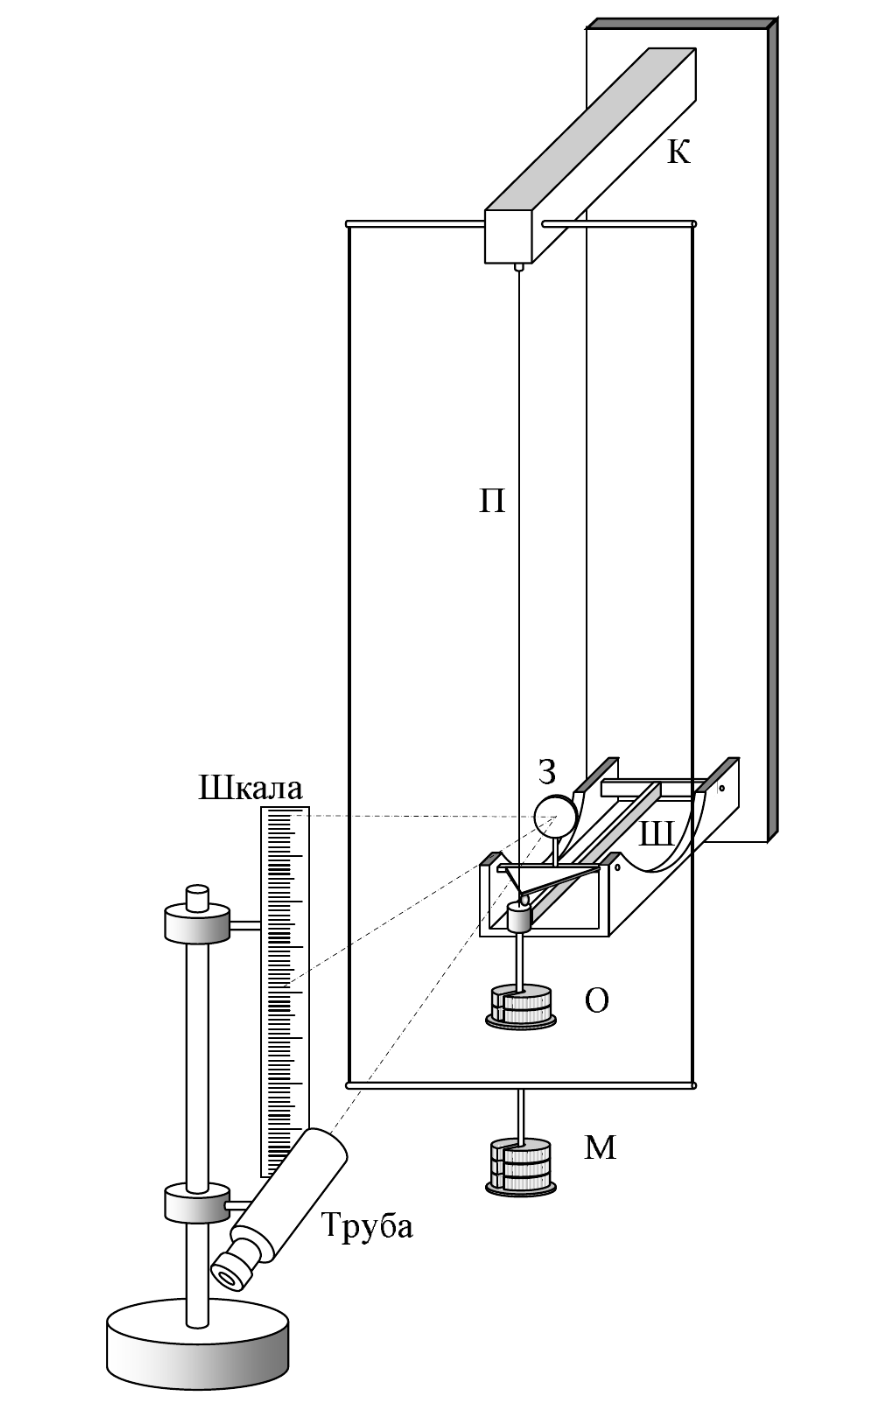
\includegraphics[scale = 0.3]{lermantov.png}
        \caption{Прибор Лермантова}
    \end{figure}

    \bigskip

    \begin{center}
    \subsection*{Погрешности}

    \begin{equation}
        \sigma_\text{сл}=\sqrt{\frac{1}{N\left( N - 1 \right)}\sum_{i=1}^{N}\left( x_\text{ср} - x_i \right)^2 }
    \end{equation}

    \begin{itemize}
	\item \textbf{Линейка:} $ \Delta_\text{лин} = 0,5 $ см
	\item \textbf{Электронные весы:} $ \Delta_\text{вес} = 0,1 $ г
    \end{itemize}

\end{center}
\end{center}

\newpage

\begin{center}
    
\section*{Ход работы}
\begin{itemize}
 
\item Данные системы: \newline 
    $ d_\text{пр} = (0,51 \pm 0,01) \text{ мм}$, $ r = (20 \pm 1) \text{ мм}$, $ l = (174,1 \pm 0,5) \text{ см}$, $ h = (144,0 \pm 0,5) \text{ см}$

\item Вычислим площадь: \newline
    $ S = \frac{\pi d_{\text{пр}^2}}{2} = 0,2042 \text{ мм}^2$, $\sigma_{S} =  2S\frac{\sigma_{d}}{d} = 0,008 \text{ мм}^2$

\item Зная предельное напряжение посчитаем максимальное давление: \newline
    $ P_{max} = 0,3 \sigma_{\text{пр}}S = 55,19 \text{ Н}$

\item Далее будет приведена таблица с измерениями. Будем последовательно класть одни и те
же грузы, потом поочередно их снимать. Проведем этот цикл 3
раза:
\end{itemize}

\end{center}

\begin{table}[H]
    \centering
    \begin{tabular}{|c|c|c|c|c|c|c|c|c|c|c|} \hline \hline
    
        $P, \text{ Н}$ & $m, \text{ г}$ & $n_1 \uparrow$, \text{ см} & $n_1 \downarrow, \text{ см}$ & $n_2 \uparrow, \text{ см}$ & $n_2 \downarrow, \text{ см}$ & $n_3 \uparrow, \text{ см}$ & $n_3 \downarrow$, \text{ см} & $l_\text{ср}, \text{ см}$ & $\sigma_{l}, \text{ см}$ \\ \hline
        4,44  & 453,3 & 15,7 & 15,8 & 15,7 & 15,8 & 15,9 & 15,9 & 15,800 & 0,036  \\ \hline
        6,85  & 245,2 & 17,7 & 17,9 & 18,0 & 18,1 & 18,2 & 18,3 & 18,033 & 0,086  \\ \hline
        9,26  & 245,3 & 19,9 & 20,1 & 20,3 & 20,3 & 20,1 & 20,2 & 20,150 & 0,061  \\ \hline
        11,66 & 244,8 & 21,8 & 22,0 & 22,1 & 22,0 & 22,1 & 22,0 & 22,000 & 0,044  \\ \hline
        14,07 & 245,9 & 23,7 & 23,8 & 23,8 & 23,8 & 23,8 & 24,0 & 23,816 & 0,040  \\ \hline
        16,48 & 245,8 & 25,4 & 25,6 & 25,5 & 25,5 & 25,6 & 25,7 & 25,550 & 0,042  \\ \hline
        18,88 & 244,9 & 27,1 & 27,3 & 27,3 & 27,5 & 27,3 & 27,4 & 27,316 & 0,054  \\ \hline
        21,29 & 245,5 & 28,8 & 28,9 & 29,0 & 29,0 & 29,0 & 29,0 & 28,950 & 0,034  \\ \hline
        23,70 & 245,3 & 30,5 & 30,9 & 30,7 & 30,7 & 30,6 & 30,6 & 30,666 & 0,055  \\ \hline
        26,11 & 245,7 & 32,2 & 32,2 & 32,2 & 32,3 & 32,4 & 32,4 & 32,283 & 0,040  \\ \hline \hline

    \end{tabular}
    \caption{Измерения}
    \label{tab:my_label}
\end{table}

\begin{center}
    Теперь по этим данным методом МНК построим график зависимости $F = kx$:
\end{center}

\begin{figure}[H]
        \centering
        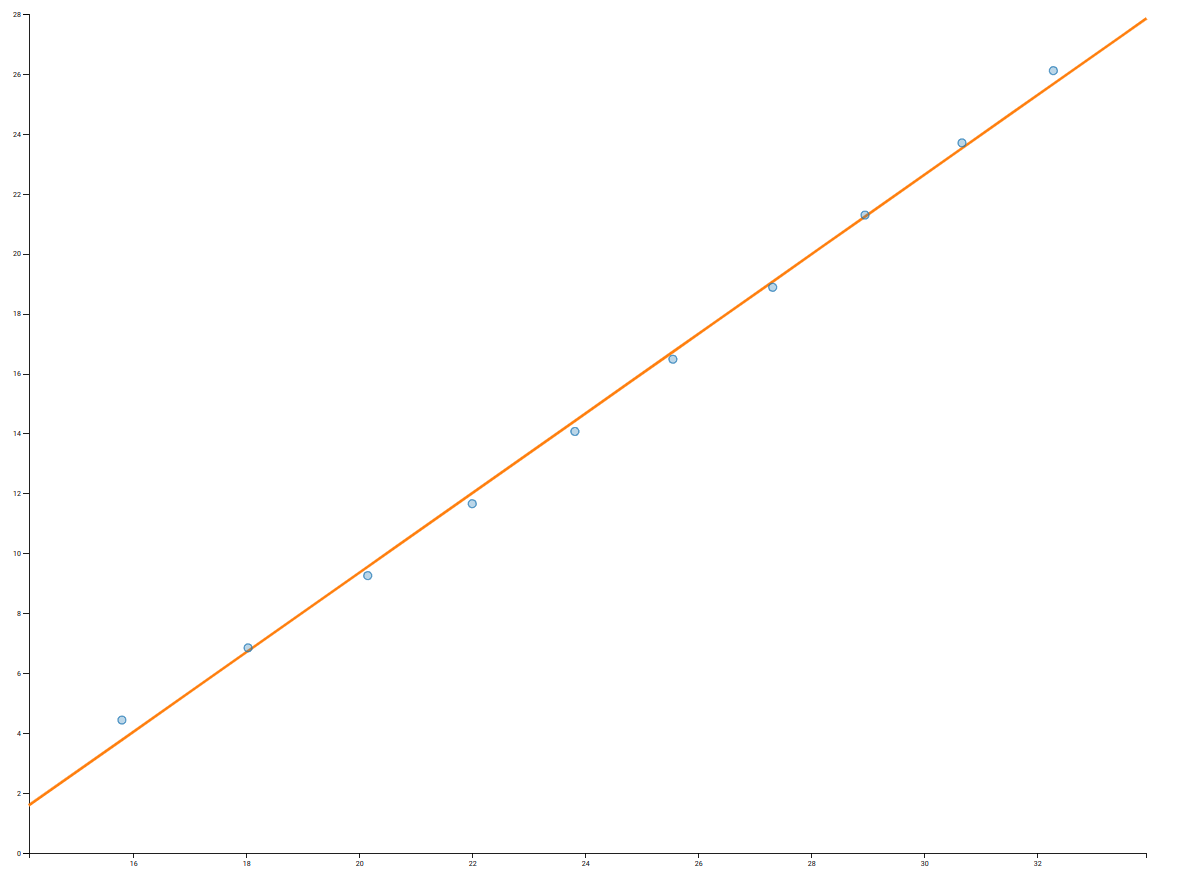
\includegraphics[scale = 0.3]{graph1.png}
        \caption{График зависимости $F = kx$}
\end{figure}

\begin{center}
    Отсюда получаем, что:
    \begin{equation}
        k = (1,708 \; \pm \; 0,890) \; \frac{\text{Н}}{\text{см}}, \; \varepsilon_{k} = 5,2 \; \% 
    \end{equation}

    \bigskip

    С учетом формул выше получаем, как выражается модуль Юнга через коэффицент наклона графика,
и выражение для его погрешности:

\begin{equation}
    \varepsilon_{E}=\sqrt{\varepsilon^2_{S}+\varepsilon^2_{k}+\varepsilon^2_{l}} \approx \varepsilon_{k} = 5,3 \%
\end{equation}

\begin{equation}
        E = \frac{kl}{S} = (145 \; \pm 7)\; \text{ГПа}
\end{equation}
\end{center}

\begin{center}

\section*{Вывод}
    
В результате работы была исследована упргуая деформация
    твердого тела. Подтверждена теоретическая модель, предсказывающая
    линейную зависимость.
\end{center}
\end{document}
